% --------------------------------------------------------------
% This is all preamble stuff that you don't have to worry about.
% Head down to where it says "Start here"
% --------------------------------------------------------------

\documentclass[12pt]{article}
\usepackage{amsmath}
\usepackage{graphicx}
\usepackage{bm}
\usepackage{float}
\usepackage{color}
\usepackage{wrapfig}
\usepackage[usenames,dvipsnames,svgnames,table]{xcolor}
\usepackage{listings}
\usepackage[margin=0.5in]{geometry}
\usepackage{booktabs}

\newcount\colveccount
\newcommand*\colvec[1]{
	\global\colveccount#1
	\begin{pmatrix}
		\colvecnext
	}
	\def\colvecnext#1{
		#1
		\global\advance\colveccount-1
		\ifnum\colveccount>0
		\\
		\expandafter\colvecnext
		\else
	\end{pmatrix}
	\fi
}

\begin{document}

% --------------------------------------------------------------
%                         Start here
% --------------------------------------------------------------

\title{G53GRA Coursework}
\author{Tom Kitchen. 4217898}

\maketitle

\lstset{language=C++,
	basicstyle=\ttfamily,
	keywordstyle=\color{teal}\ttfamily,
	stringstyle=\color{red}\ttfamily,
	commentstyle=\color{blue}\ttfamily,
	morecomment=[l][\color{magenta}]{\#}}

\section{Coursework}
\subsection*{Introduction}

My coursework attempts to recreate a stadium at a Judo competition. In judo, competitors aim to win by throwing their opponent onto their back. In my scene you see the opening and closing sequence of a judo match. The competitors bow as they enter the arena, bow before they fight, after they fight and finally as they leave the arena. As a display of respect competitors never turn their back on one another.

\subsection{Making the players: Hierarchical Modelling and Animation }
The players are built using hierarchical modelling. The model allows us to specify the angles of the players joints. 

\subsubsection{Calculating the correct position of the Person}

\begin{wrapfigure}{r}{0.3\textwidth}
\centering
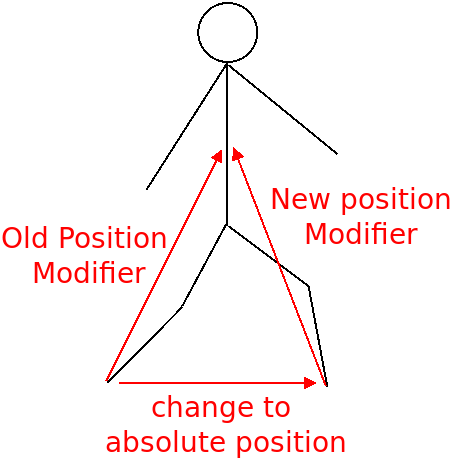
\includegraphics[width=0.3\textwidth]{posmod.png}
\end{wrapfigure}
This was one of the more complicated parts of the code. For example when animating walking, the foot touching the ground should stay in the same place throughout the step. To calculate the position of the player I had to calculate the difference in position between the foot and the centre of the body (which the hierarchical model used as the reference point). I called this quantity the position modifier. When the player takes a step the reference point changes. To compensate for this the code calculates the new position modifier from the other foot, and set the position to old position + old position modifier to new position modifier. 
\subsubsection{Animating the person: Interpolation}
To create animation I used interpolation similar to that in the Pixar lamp example. For each action keyframes are defined and the program interpolates between the keyframes. 

\subsection{Viewing / User controls}

\subsubsection{Bounding viewing position}
I limited the camera position to only allow locations within the Scene. This means a user can't accidentally leave the Scene and see things that I didn't indent them to.

\subsubsection{First and Third Person modes}

I modified the camera class to allow it to store pointers to other objects. I edited the camera object to set its position and direction to the position of the chosen object. You can view in first person mode with the p key and third person with the o key. The i key resets this.

A view of first person mode (left), and third person (right) is demonstrated.


\begin{center}
	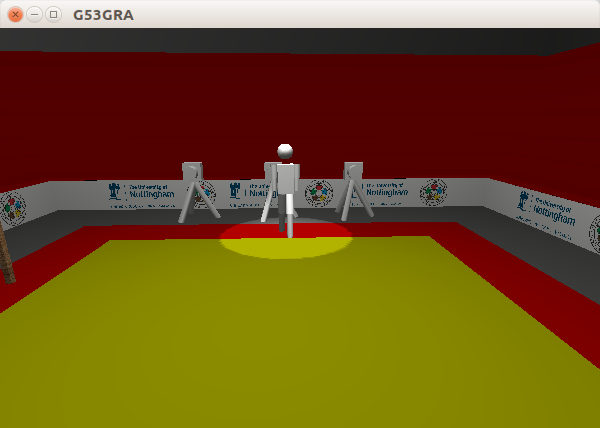
\includegraphics[width=0.8\textwidth]{FirstPerson.png} 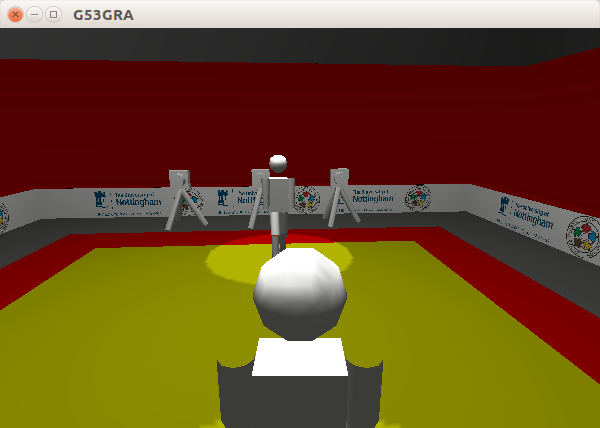
\includegraphics[width=0.8\textwidth]{ThirdPerson.png}
\end{center}


\subsection{Texturing}
 One feature you always see at sporting evens is sponsorship banners in the arena. I used texturing to create this kind of effect. 
 
 I added a wood texture to the table and chairs.
 
 I used texture files to emulate the clothing. The officials wear suits while the competitors wear blue and white judogis. 
\begin{center}
 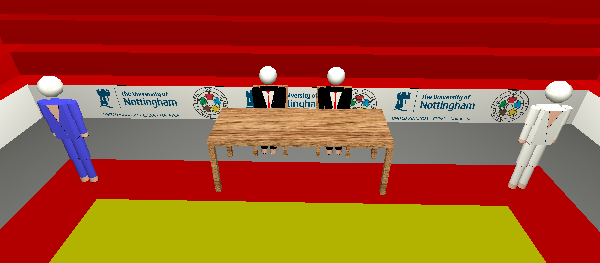
\includegraphics[width=0.8\textwidth]{Texturing.png}
\end{center}


\subsection{Lighting}

The lighting consisted of two components, a background light that was similar to the examples studied in lectures, and spotlights which followed the players as they walked into the arena.



\begin{center}
	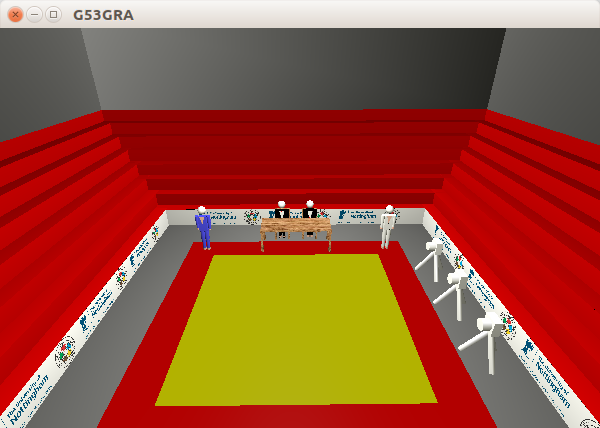
\includegraphics[width=0.8\textwidth]{Arena.png}
\end{center}


\subsubsection{Spotlights that follow the characters motion}
This involved storing a pointer to the player object in a spotlight object. Simple trigonometry allows us to work out the correct angle to point the spotlight to follow the player. I opted to dim the main lights and turn on the spotlights when the players enter/leave the mat to bring focus to them.

\begin{center}
	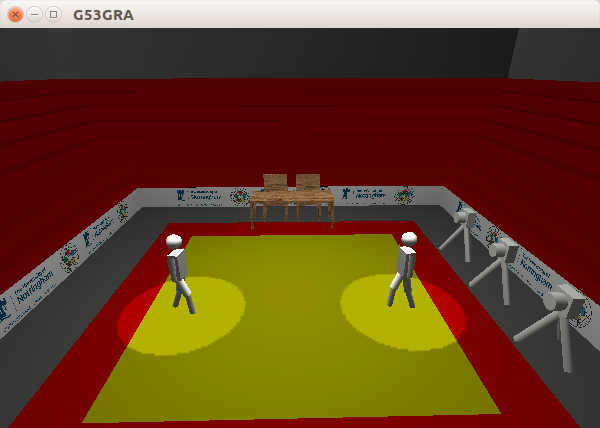
\includegraphics[width=0.8\textwidth]{Spotlights.png}
\end{center}







\end{document}
